\chapter*{Introduction}
\addcontentsline{toc}{chapter}{Introduction}

Audio processing involves the manipulation and analysis of sound signals to enhance, modify, or analyze the audio data. This incorporates a wide range of techniques and algorithms. The types of audio signals categorize the audio processing into analog and digital processing. In the context of sound source localization, the settings mostly refer to the digital audio signal analysis.

Sound source localization (SSL) is the process of identifying the relative location of one or multiple sound sources in a given environment with various acoustic signals \cite{desai_review_2022}. This technique plays a significant role in acoustic signal processing, enabling the system to interpret the audio information spatially.

\begin{figure}[h]
    \centering
    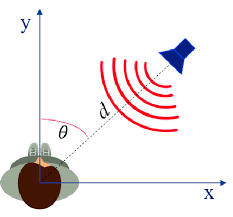
\includegraphics[width=0.3\linewidth]{figures/SSL_Explain.png}
    \caption{Principle of SSL}
    % \label{fig:enter-label}
\end{figure}

The SSL methods mostly utilize a microphone array that contains multiple microphones for source localization purposes, which is similar to other signal positioning systems, the Global Navigation Satellite System (GNSS) as an example, and is hardly achievable by using a single signal receiver. In this project, the SSL process will be conducted using a multi-microphone array.

\begin{figure}[h]
    \centering
    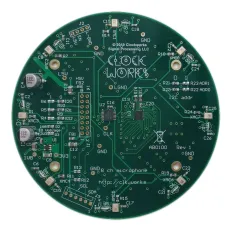
\includegraphics[width=0.3\linewidth]{figures/Microphone_Array1.png}
    \caption{An Example of 8-Channels Microphone Array}
    % \label{fig:enter-label}
\end{figure}

When considering the transmission of sound waves in space, the process can usually be described by two different models: the near-field model and the far-field model \cite{westervelt_parametric_1963}. The near-field model refers to scenarios where the distance between the sound source and the microphone array is short, resulting in sound waves being treated as spherical waves. Conversely, the far-field model applies when the distance is sufficiently large to consider the sound waves as plane waves. In the following studies, the far-field condition will be applied to all situations.

Traditionally, the SSL problems can be resolved in various ways. These methods typically estimate the direction of arrival (DoA) of the sound signal using mathematical models. However, limitations exist among these methods. For example, conventional approaches like multiple signal classification (MUSIC) have limitations in processing overlapping sound sources and noisy scenarios \cite{limitation_MUSIC_2021}.

\begin{figure}[h]
    \centering
    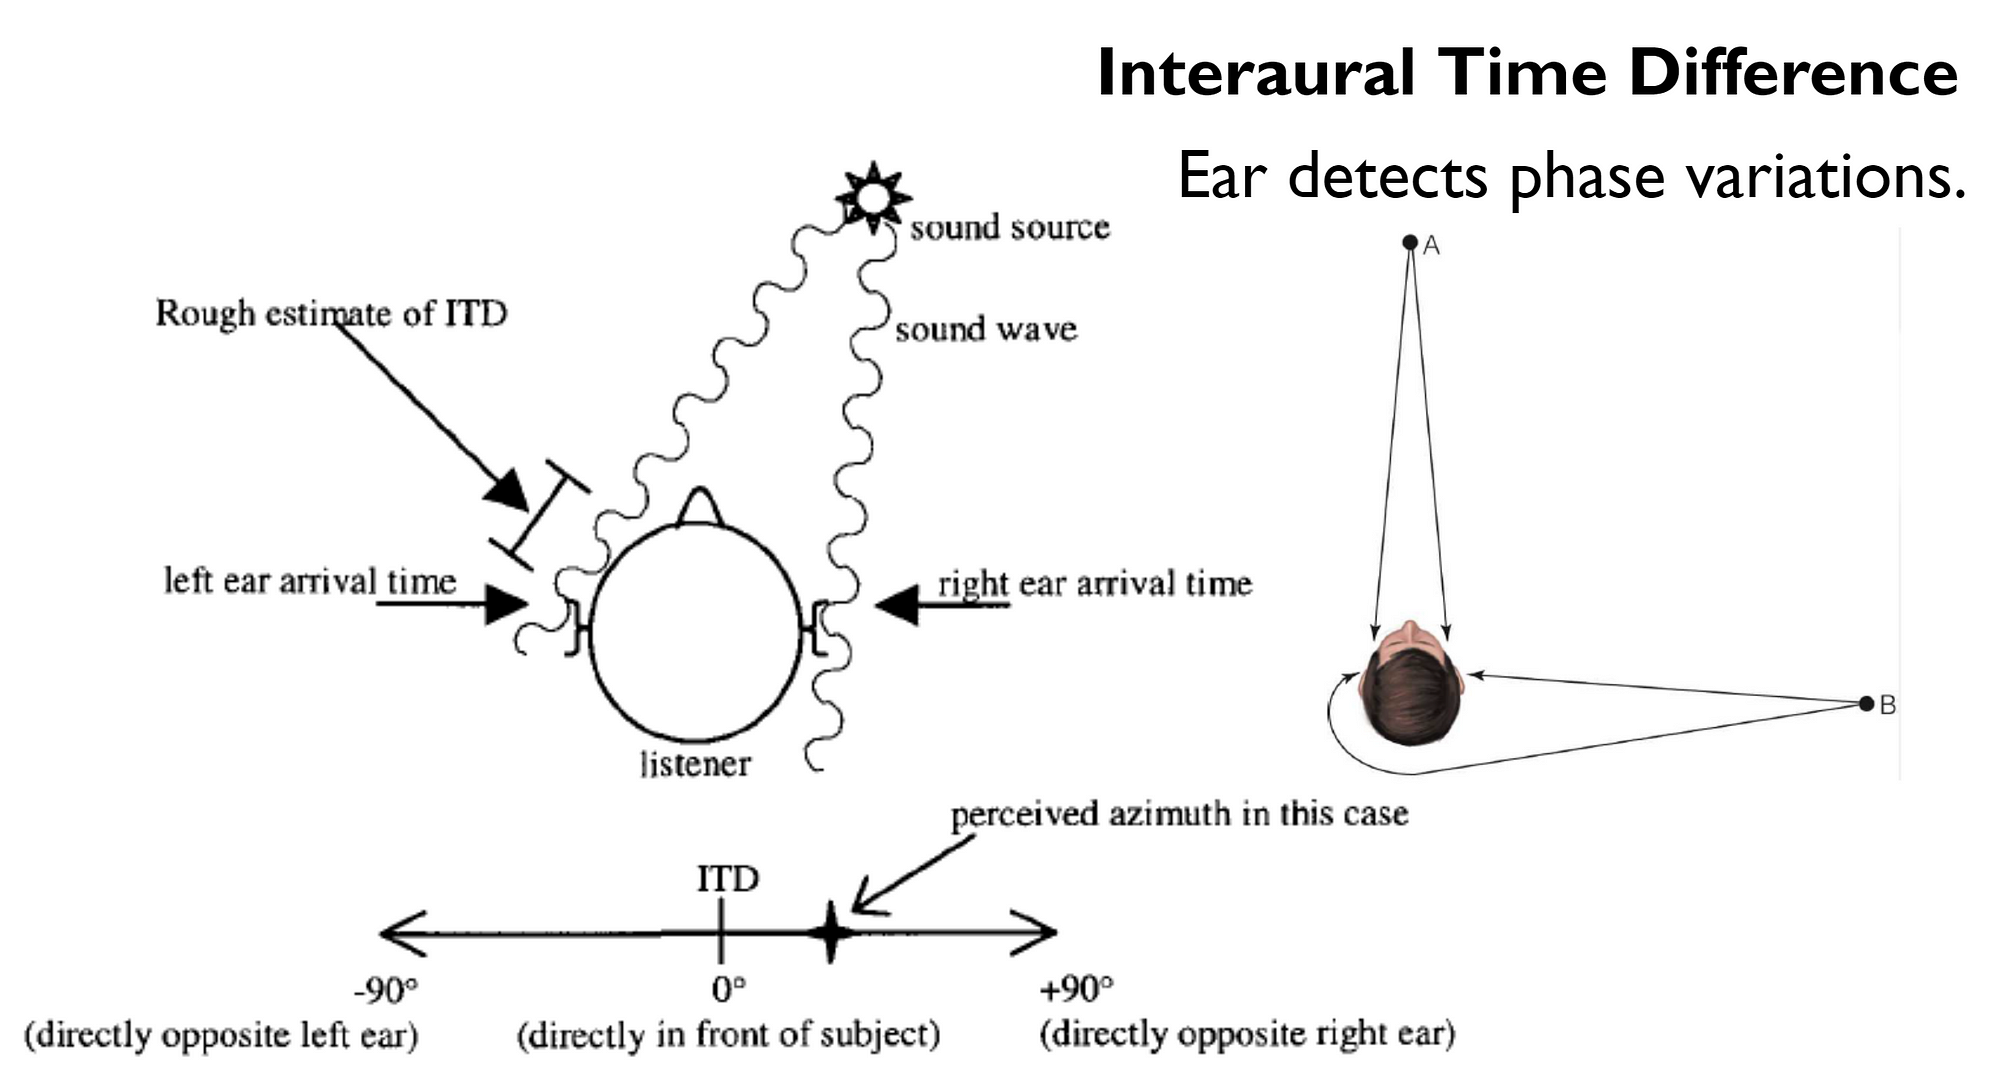
\includegraphics[width=0.5\linewidth]{figures/Human_Ears_TDOA.png}
    \caption{Human Ears Provide a Typical Example of TDOA}
    % \label{fig:enter-label}
\end{figure}

In recent years, deep learning (DL) has emerged as a branch of machine learning, being an innovative solution to robot perceptual problems. By utilizing large datasets and neural network architectures, deep learning models, often referred to as deep neural networks (DNN), can extract relevant information and features from the original audio signals, either directly or indirectly, without the need of physical-meaning-based mathematical models. DL techniques such as convolutional neural networks (CNNs) and recurrent neural networks (RNNs) have already demonstrated promising results in the audio processing area, overcoming several limitations in the traditional algorithms such as the noise and reverberation problems in a given environment.

 One of the most significant SSL applications is robotic perception since understanding the location of sounds can enhance robots' navigation capabilities, especially for non-stationary obstacle identification abilities. However, different from the situation of SSL in the laboratory context, SSL perception for robots requires high robustness, computational efficiency, and adaptivity to complex environments.





















% \section{Section}
% \subsection{Subsection}
% \subsubsection{Subsubsection}
% \lipsum[1-5] \parencite{cicero1883finibus}

% \begin{figure}[ht]
%     \centering
%     
\includegraphics[width = 0.5\textwidth]{PolyU.png}
%     \caption{The Hong Kong Polytechnic University}
%     \label{PolyU}
% \end{figure}

% \begin{table}[ht]
%     \centering
%     \begin{tabular}{l|l}
%     \toprule
%          This & is \\ \midrule
%          a & table.\\ \bottomrule
%     \end{tabular}
%     \caption{A table}
%     \label{Table}
% \end{table}

